%%%%%%%%%%%%%%%%%%%%%%%%%%%%%%%%%%%%%%%%%%%%%%%%%%%%%%%%%%%%%%%%%%%%%%%%%%%%%%%%
%2345678901234567890123456789012345678901234567890123456789012345678901234567890
%        1         2         3         4         5         6         7         8

\documentclass[letterpaper, 10 pt, conference]{ieeeconf}  % Comment this line out if you need a4paper

%\documentclass[a4paper, 10pt, conference]{ieeeconf}      % Use this line for a4 paper

\IEEEoverridecommandlockouts                              % This command is only needed if 
                                                          % you want to use the \thanks command

\overrideIEEEmargins                                      % Needed to meet printer requirements.

%In case you encounter the following error:
%Error 1010 The PDF file may be corrupt (unable to open PDF file) OR
%Error 1000 An error occurred while parsing a contents stream. Unable to analyze the PDF file.
%This is a known problem with pdfLaTeX conversion filter. The file cannot be opened with acrobat reader
%Please use one of the alternatives below to circumvent this error by uncommenting one or the other
%\pdfobjcompresslevel=0
%\pdfminorversion=4

% See the \addtolength command later in the file to balance the column lengths
% on the last page of the document

% The following packages can be found on http:\\www.ctan.org
\usepackage{graphics} % for pdf, bitmapped graphics files
\usepackage{graphicx} 
%\usepackage{epsfig} % for postscript graphics files
% \usepackage{mathptmx} % assumes new font selection scheme installed
%\usepackage{times} % assumes new font selection scheme installed
\usepackage{amsmath} % assumes amsmath package installed
% \usepackage{amssymb}  % assumes amsmath package installed
\usepackage{multirow}
\usepackage{amsfonts}
\usepackage{xcolor}


\title{\LARGE \bf
Evaluating the Optimality of Reinforcement Learning Using Input Shaping
}


\author{Albert Author$^{1}$ and Bernard D. Researcher$^{2}$% <-this % stops a space
\thanks{*This work was not supported by any organization}% <-this % stops a space
\thanks{$^{1}$Albert Author is with Faculty of Electrical Engineering, Mathematics and Computer Science,
        University of Twente, 7500 AE Enschede, The Netherlands
        {\tt\small albert.author@papercept.net}}%
\thanks{$^{2}$Bernard D. Researcheris with the Department of Electrical Engineering, Wright State University,
        Dayton, OH 45435, USA
        {\tt\small b.d.researcher@ieee.org}}%
}


\begin{document}



\maketitle
\thispagestyle{empty}
\pagestyle{empty}


%%%%%%%%%%%%%%%%%%%%%%%%%%%%%%%%%%%%%%%%%%%%%%%%%%%%%%%%%%%%%%%%%%%%%%%%%%%%%%%%
\begin{abstract}

Legged mobile robotic systems are often deployed because of their many advantages over wheeled or tracked systems. They have been shown to be able to traverse more treacherous terrain deploying jumping-like techniques to overcome otherwise not traversable landscapes. It is difficult however to define robust and efficient control strategies for these types of systems using traditional methods however. Using input shaping techniques, it has been shown that optimal jumping strategies can be defined for flexible systems. In this work, input shaping is used to validate if reinforcement learning can find similar optimal jumping techniques using a monopode jumping system.

\end{abstract}


%%%%%%%%%%%%%%%%%%%%%%%%%%%%%%%%%%%%%%%%%%%%%%%%%%%%%%%%%%%%%%%%%%%%%%%%%%%%%%%%
\section{INTRODUCTION}
\subsection{Legged Locomotion}

Using legged mobile systems as compared to wheeled or tracked systems is often advantageous in terms of system capability. These systems have been used for their ability to navigate harsh, uneven and unpredictable terrain \cite{}. Defining control strategies for these systems is challenging however particularly when flexible components are introduced into the morphology. Many techniques exist to define locomotion strategies still, many of which are considered traditional \cite{}. Modern machine learning methods such as reinforcement learning have also shown promise in their ability to define proper control strategies.

\subsection{Reinforcement Learning}
Reinforcement learning, a form of machine learning, has been shown to be a viable method for defining controllers for many different types of systems \cite{}. In particular, the method has proven useful for learning complex control inputs for robotics systems /cite{}. Though many different types of algorithms have been evaluated, the ones that are most prevalent in regards to the ability to consistently learn without strenuous hypermeter tuning are actor-critic and gradient decent type algorithms. 

The challenge of tuning an algorithm to find control strategies is not negated all together though, particularly when training a robust controller expected to perform with unexpected physical changes to the system. Training utilizing domain randomization has been shown to improve controller performance where system mechanical parameters may experience inaccuracies \cite{}. In addition, this technique has been shown to be useful when performing the simulation-to-real process \cite{}. In this work it is of interest to discover how the utilization of domain randomization changes the controller's output when changing system parameters. 

Of the different algorithms currently considered cutting-edge in research, Twin Delayed Deep Deterministic Policy Gradient (TD3) is one which has shown its ability for robotics control systems \cite{}. This algorithm, being built from the popular Deep Deterministic Policy Gradient (DDPG) \cite{}, and is of the actor-critic type. TD3 was the algorithm of choice and was used to train all the controllers in this work. Details regarding the specifics behind the algorithm and the training parameters are highlighted in the \textbf{Appendix}.

\subsection{Input Shaping}
\textcolor{red}{Some background information on input shaping. Some words from DVs paper.}

\section{ENVIRONMENT}
%
\begin{figure}[t]
        \begin{center}
        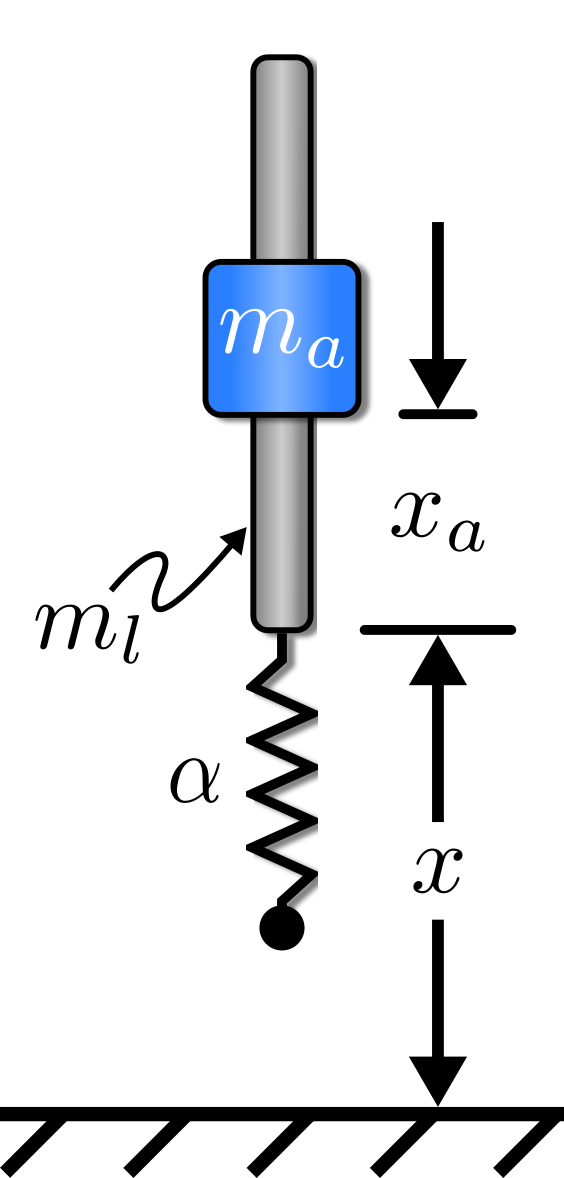
\includegraphics[width=0.15\textwidth]{figures/Monoped_System/monoped.png}
        \caption{Pogo-stick System}
        \label{fig:pogoStickSystem} 
        \end{center}
\end{figure}
%
\begin{table}[t]
        \caption{Pogo-stick Model Parameters}
        \vspace{-4mm}
        \label{tab:pogoStickSystem}
        \begin{center}
                \begin{tabular}{c c}
                %			& & \\ % put some space after the caption
                \hline
                \hline
                \textbf{Model Parameter} & \textbf{Value}\\
                \hline
                Mass of Leg, $m_l$                                       & 0.175 kg                                          \\
                Mass of Actuator, $m_a$                                  & 1.003 kg                                          \\
                Spring Constant, $\alpha_{nominal}$                      & 5760 $\textup{N}/\textup{m}$                      \\
                Natural Frequency, $\omega_n$                            & $\sqrt{\frac{\alpha}{m_l + m_a}}$                 \\
                Damping Ratio, $\zeta_{nominal}$                         & 1e-2 $\frac{\textup{N}}{\textup{m/s}}$            \\
                Gravity, $g$                                             & 9.81 m/s$^2$                                      \\
                \hline
                Actuator Stroke, $(x_{a})_{\textup{max}}$                & 0.008 $\textup{m}$                                \\
                Max.\ Actuator Velocity, $(\dot{x}_{a})_{\textup{max}}$  & 1.0 $\textup{m}/\textup{s}$                       \\ 
                Max.\ Actuator Acceleration, $(\ddot{x}_{a})_{\textup{max}}$   & 10.0 $\textup{m}/\textup{s}^2$                    \\
                \hline
                \hline
                \end{tabular}
        \end{center}
\end{table}
% 
Controlling the system is done so by accelerating the mass of the actuator $m_a$ along the mass of the rod $m_l$. A nonlinear spring with constant $\alpha$ is modeled to represent system flexibility along with a damper (not shown in figure). The variables $x$ and $x_a$ represent the rod's position from zero and the actuator's position along the rod, respectively.

The equations which govern system behavior in simulation are: 
% 
\begin{equation}
        \label{eq:EOM}
        \begin{aligned}
            \ddot{x} = \frac{\gamma}{m_t} \left(\alpha\,x + \beta\,x^3 + c\,\dot{x}\right)-\frac{m_a}{m_t}\,\ddot{x}_a-g
        \end{aligned}
\end{equation}
% 
where $\ddot{x}$, $\dot{x}$ and $x$ are the rod's acceleration, velocity and position, respectively; $\ddot{x}$ represents the actuator acceleration and system input. The system's total mass along with the actuator's mass are represented by $m_t$ and $m_a$, respectively. Constants $c$ and $a$ represent the damping ratio and spring constant, and $\beta$ is set to $1e8$. Constant $\gamma$ is in place to prevent the system's spring and damper from acting when the system is not in contact with the ground and can be expressed as:
% 
\begin{equation}
        \label{eq:EOMgama}
        \begin{aligned}
                \gamma =
                \left\{\begin{matrix}
                    -1, & x \leq 0\\ 
                    \hphantom{-} 0, & \textup{otherwise}
                \end{matrix}\right.
        \end{aligned}
\end{equation}
% 
The spring compression limit, or the systems position in the negative $x$ direction, is limited to 0.008m. Additionally, the system is confined to move only vertically in regards to Fig.~\ref{} so that controlling ballance is not required.

\section{Method}

\subsection{Environment Setup}
% 
\begin{figure}[t]
        \begin{center}
        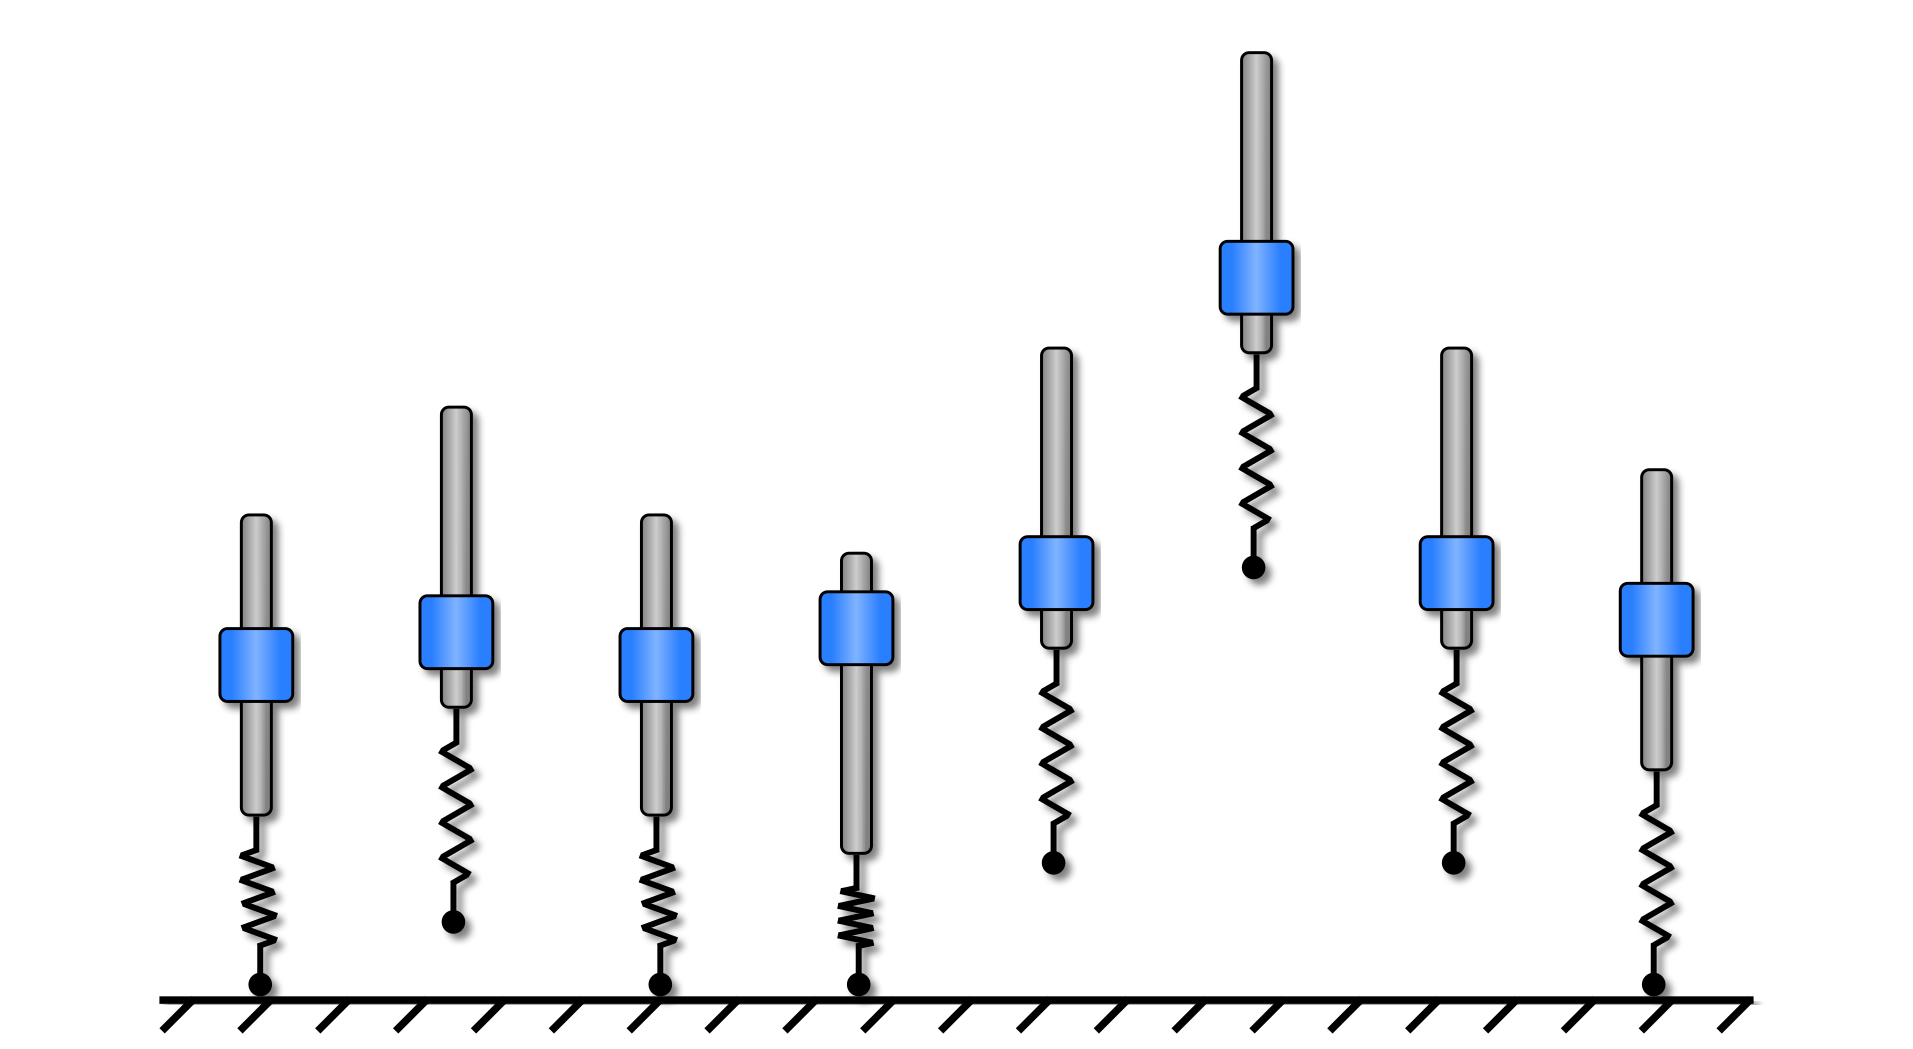
\includegraphics[width=0.45\textwidth]{figures/Monoped_System/stutter_jump.png}
        \caption{Example Stutter Jump}
        \label{fig:stutterJump} 
        \end{center}
\end{figure}
% 
One hundred controllers were trained for each case discussed below, each with a different network initialization based on a set of seeds. This was to ensure the methods were reliable and repeatable. The network seeds used in this work can be found in the **Appendix**. The controllers were trained to jump in a manner matching what is seen in Fig.~\ref{}. This type of jump has been called a stutter jump and can be described as the system jumping firstly to gain energy and secondly to gain height.

The state space and action space which the TD3 algorithm was provided was:
%
\begin{equation}
        \label{eq:stateSpace}
        \begin{aligned}
                \mathcal{S} = \left[ x_{a_t}, \dot{x}_{a_t}, x_t, \dot{x}_t \right]
        \end{aligned}
\end{equation}
%     
\begin{equation}
        \label{eq:stateSpace}
        \begin{aligned}
                \mathcal{A} = [\ddot{x}_{a_t}]
        \end{aligned}
\end{equation}
%
where $x_{a_t}$ and $\dot{x}_{a_t}$ are the actuator's position and velocity, respectively, and $x_{t}$ and $\dot{x}_{t}$ are the rod's position and velocity, respectively. $\ddot{x}_{a_t}$ is the actuator's acceleration and the system input.

\textcolor{red}{Table of System Initial Position}

At the start of each training episode, the system was initialized according to states provided in Tab.~\ref{}. The rod's position was set accounting for spring compression due to system mass so that the system was at rest. The actuator was initialized randomly along its full length stroke. See Section.~\ref{} and Section.~\ref{} for further details on the mechanical parameters changed during simulation initialization.

A training episode was considered completed if one of two parameters where met. Either the system completed a stutter jump, where the rod's position became greater than zero and then returned to zero twice, or the episode reached the maximum number of steps. In this work, the maximum number of steps was set to 500 which represented a 5 second simulation.

\subsection{Non Robust}
The controllers trained in a non-robust fashion were done so without deploying domain randomization. Therefore the system was initialized with the same set of mechanical parameters for each episode. Those parameters are highlighted in Tab.~\ref{}. The rewards passed to the TD3 algorithm were design to test two learning scenarios: learning to jump as high as possible and learning to jump as high as possible efficiently. The rewards used were:

\begin{equation}
        \label{eq:rewardHeight}
        \begin{aligned}
                R_{height} = x_t
        \end{aligned}
\end{equation}
%
\begin{equation}
        \label{eq:rewardEfficiency}
        \begin{aligned}
                R_{efficiency} = \frac{x_t}{\sum P_t}
        \end{aligned}
\end{equation}

where, $x_t$ and $P_t$ were the rod's height and the system't power used at each time step, respectively. Power usage in this work was defined mechanically as the product of the actuator's mass, acceleration and velocity. 

\begin{itemize}
        \item Deploy TD3 (maybe PPO as well) to train agents to
        \item Jump to maximum height
        \item Jump to specified height
        \item Jump to max/specified height efficiently
\end{itemize}

\subsection{Robust}
The controllers trained to be able to combat changes in system parameters were trained employing domain randomization. The spring constant, $k$, was randomly initialized at the start of each episode such that the natural frequency of the system could change by $\pm\,30 \%$. Additionally, the damping ratio, $\zeta$, was randomly set between the ranges of $0.00$ and $0.01$, where the expectation was lower $\zeta$ values would lead to better performance both in height and efficiency. The rewards used to train the robust controllers were the same as the non-robust controllers and can be seen in Eq.~\ref{} and Eq.~\ref{}. 

\begin{itemize}
        \item Deploy TD3 (maybe PPO as well) to train agents to
        \item Jump to maximum height
        \item Jump to specified height
        \item Jump to max/specified height efficiently
\end{itemize}

\subsection{Input Shaping}
How were the commands generated?

\begin{itemize}
        \item Jump to maximum height
        \item Jump to specified height
        \item Jump to specified height efficiently
        \item Perform different jump types
        \item Single jump
        \item Stutter jump
\end{itemize}


\section{RESULTS}
\subsection{Controller Trained to be Non-Robust}
\begin{itemize}
        \item Figure: Input of all three methods
        \item Figure: Jumping Height of all three methods
        \item Figure: Power usage scatter chart of all three methods
\end{itemize}

\subsection{Controller Trained to be Robust}
\begin{itemize}
        \item Figure: Input of all three methods
        \item Figure: Power usage scatter chart of all three methods
        \item Figure: Jumping Height of all three methods
\end{itemize}

\section{CONCLUSION}
A conclusion section is not required. Although a conclusion may review the main points of the paper, do not replicate the abstract as the conclusion. A conclusion might elaborate on the importance of the work or suggest applications and extensions. 

\addtolength{\textheight}{-12cm}   % This command serves to balance the column lengths
                                  % on the last page of the document manually. It shortens
                                  % the textheight of the last page by a suitable amount.
                                  % This command does not take effect until the next page
                                  % so it should come on the page before the last. Make
                                  % sure that you do not shorten the textheight too much.

%%%%%%%%%%%%%%%%%%%%%%%%%%%%%%%%%%%%%%%%%%%%%%%%%%%%%%%%%%%%%%%%%%%%%%%%%%%%%%%%



%%%%%%%%%%%%%%%%%%%%%%%%%%%%%%%%%%%%%%%%%%%%%%%%%%%%%%%%%%%%%%%%%%%%%%%%%%%%%%%%



%%%%%%%%%%%%%%%%%%%%%%%%%%%%%%%%%%%%%%%%%%%%%%%%%%%%%%%%%%%%%%%%%%%%%%%%%%%%%%%%
\section*{APPENDIX}
\subsection*{Twin Delayed Deep Deterministic Policy Gradient (TD3)} 

TD3 is an actor-critic, off-policy reinforcement learning algorithm wherein the controller is represented by the actor which is formally know as the policy $\pi_{\phi}$. In the deep learning case, the actor is a neural network. The actor takes actions, $\mathcal{A}$, at each time step during simulation which are the system's inputs. The critic is represented by the estimated expected return of taking action $\mathcal{A}$ in state $\mathcal{S}$ and following the policy $\pi$ from then after. The critic is also a neural network, and it is updated according to the temporal difference error found between a set of twin target networks. These target networks are updated to follow the critic network every defined $n$ updates of the critic network. The hyperameters used for the experiments in this work can be found in Table~\ref{}.

\textcolor{red}{Table of Hyperparameters}

\subsection*{Network Initialization Seeds}
When training a neural network from scratch, once the network design is defined, the node weights must be initialized. In this work, 100 different controllers were trained each with a different network initialization based on a set of seeds. The seeds are listed in Tab.~\ref{}.

\textcolor{red}{Table of Network Seeds}

\section*{ACKNOWLEDGMENT}

The authors would like to thank the Louisiana Crawfish Promotion and Research Board for their support of this work.


%%%%%%%%%%%%%%%%%%%%%%%%%%%%%%%%%%%%%%%%%%%%%%%%%%%%%%%%%%%%%%%%%%%%%%%%%%%%%%%%

References are important to the reader; therefore, each citation must be complete and correct. If at all possible, references should be commonly available publications.



\begin{thebibliography}{99}

\bibitem{c1} G. O. Young, 'Synthetic structure of industrial plastics (Book style with paper title and editor),' 	in Plastics, 2nd ed. vol. 3, J. Peters, Ed.  New York: McGraw-Hill, 1964, pp. 15'64.
\bibitem{c2} W.-K. Chen, Linear Networks and Systems (Book style).	Belmont, CA: Wadsworth, 1993, pp. 123'135.
\bibitem{c3} H. Poor, An Introduction to Signal Detection and Estimation.   New York: Springer-Verlag, 1985, ch. 4.
\bibitem{c4} B. Smith, 'An approach to graphs of linear forms (Unpublished work style),' unpublished.
\bibitem{c5} E. H. Miller, 'A note on reflector arrays (Periodical style'Accepted for publication),' IEEE Trans. Antennas Propagat., to be publised.
\bibitem{c6} J. Wang, 'Fundamentals of erbium-doped fiber amplifiers arrays (Periodical style'Submitted for publication),' IEEE J. Quantum Electron., submitted for publication.
\bibitem{c7} C. J. Kaufman, Rocky Mountain Research Lab., Boulder, CO, private communication, May 1995.
\bibitem{c8} Y. Yorozu, M. Hirano, K. Oka, and Y. Tagawa, 'Electron spectroscopy studies on magneto-optical media and plastic substrate interfaces(Translation Journals style),' IEEE Transl. J. Magn.Jpn., vol. 2, Aug. 1987, pp. 740'741 [Dig. 9th Annu. Conf. Magnetics Japan, 1982, p. 301].
\bibitem{c9} M. Young, The Techincal Writers Handbook.  Mill Valley, CA: University Science, 1989.
\bibitem{c10} J. U. Duncombe, 'Infrared navigation'Part I: An assessment of feasibility (Periodical style),' IEEE Trans. Electron Devices, vol. ED-11, pp. 34'39, Jan. 1959.
\bibitem{c11} S. Chen, B. Mulgrew, and P. M. Grant, 'A clustering technique for digital communications channel equalization using radial basis function networks,' IEEE Trans. Neural Networks, vol. 4, pp. 570'578, July 1993.
\bibitem{c12} R. W. Lucky, 'Automatic equalization for digital communication,' Bell Syst. Tech. J., vol. 44, no. 4, pp. 547'588, Apr. 1965.
\bibitem{c13} S. P. Bingulac, 'On the compatibility of adaptive controllers (Published Conference Proceedings style),' in Proc. 4th Annu. Allerton Conf. Circuits and Systems Theory, New York, 1994, pp. 8'16.
\bibitem{c14} G. R. Faulhaber, 'Design of service systems with priority reservation,' in Conf. Rec. 1995 IEEE Int. Conf. Communications, pp. 3'8.
\bibitem{c15} W. D. Doyle, 'Magnetization reversal in films with biaxial anisotropy,' in 1987 Proc. INTERMAG Conf., pp. 2.2-1'2.2-6.
\bibitem{c16} G. W. Juette and L. E. Zeffanella, 'Radio noise currents n short sections on bundle conductors (Presented Conference Paper style),' presented at the IEEE Summer power Meeting, Dallas, TX, June 22'27, 1990, Paper 90 SM 690-0 PWRS.
\bibitem{c17} J. G. Kreifeldt, 'An analysis of surface-detected EMG as an amplitude-modulated noise,' presented at the 1989 Int. Conf. Medicine and Biological Engineering, Chicago, IL.
\bibitem{c18} J. Williams, 'Narrow-band analyzer (Thesis or Dissertation style),' Ph.D. dissertation, Dept. Elect. Eng., Harvard Univ., Cambridge, MA, 1993. 
\bibitem{c19} N. Kawasaki, 'Parametric study of thermal and chemical nonequilibrium nozzle flow,' M.S. thesis, Dept. Electron. Eng., Osaka Univ., Osaka, Japan, 1993.
\bibitem{c20} J. P. Wilkinson, 'Nonlinear resonant circuit devices (Patent style),' U.S. Patent 3 624 12, July 16, 1990. 

\end{thebibliography}

\end{document}
